%--------------------------------------------------------------- %
\documentclass[SPC-MASTER.tex]{subfiles}
\begin{document}
	\Large
	
\section{Individual/Moving-Range chart}
% http://en.wikipedia.org/wiki/Shewhart_individuals_control_chart
\begin{itemize}
\item The individual/moving-range chart is a type of control chart used to monitor variables data from a business or industrial process for which it is impractical to use rational subgroups.

\item The chart is necessary in the following situations:
\begin{itemize}
\item[$\ast$] Where automation allows inspection of each unit, so rational subgrouping has less benefit.
\item[$\ast$]Where production is slow so that waiting for enough samples to make a rational subgroup unacceptably delays monitoring
\item[$\ast$] For processes that produce homogeneous batches (e.g., chemical) where repeat measurements vary primarily because of measurement error
\end{itemize}
\item The "chart" actually consists of a pair of charts: one, the individuals chart, displays the individual measured values; the other, the moving range chart, displays the difference from one point to the next. 
\item As with other control charts, these two charts enable the user to monitor a process for shifts in the process that alter the mean or variance of the measured statistic.
\end{itemize}
\begin{figure}[h!]
\centering
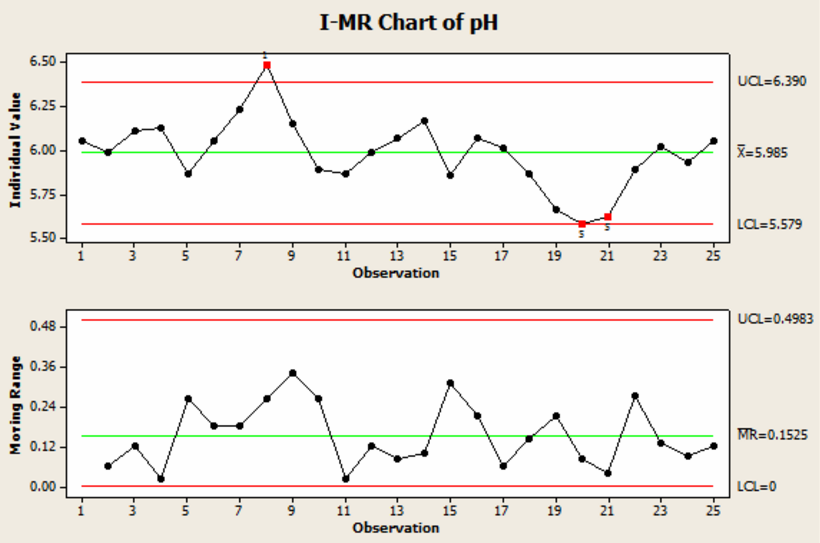
\includegraphics[width=0.7\linewidth]{images/IMRChart}
\caption{}
\label{fig:imrchart}
\end{figure}


\end{document}